\section{Introduction}

\begin{definition}[\textit{Computer performance}]
    Computer performance refers to the overall effectiveness of a computer system, taking into account factors such as throughput, individual response time, and availability.
\end{definition}
It can be measured by assessing the amount of useful work that a computer system or network can accomplish in a given amount of time and resources.

Commonly, systems are predominantly validated against functional requirements rather than quality ones. 
Ensuring quality needs different skills, which can be hard to find. 
There's a trend to hurry products to market quickly, making them seem more appealing. 
Early on, there's often not much info about quality, but understanding it is crucial for cost and performance.
This matters not just when designing and sizing the system but also as it evolves over time.

\subsection{System quality evaluation}
\paragraph*{Intuition and trends evaluation}
Intuition and trend extrapolation involve making quick and flexible assessments based on gut feelings and projected patterns. 
However, individuals with sufficient expertise in these areas are rare, and the accuracy of their predictions may sometimes be questionable.
\paragraph*{Experimental evaluation}
Assessing alternatives through experimentation can be highly beneficial, and at times, it's the preferred method. 
However, it can also be costly, sometimes excessively so. 
Another downside is that experiments may only provide detailed insights into system behavior under specific conditions, lacking broader generalizations.
On the upside, they tend to offer excellent accuracy, albeit at the expense of being labor-intensive and less adaptable.
\begin{figure}[H]
    \centering
    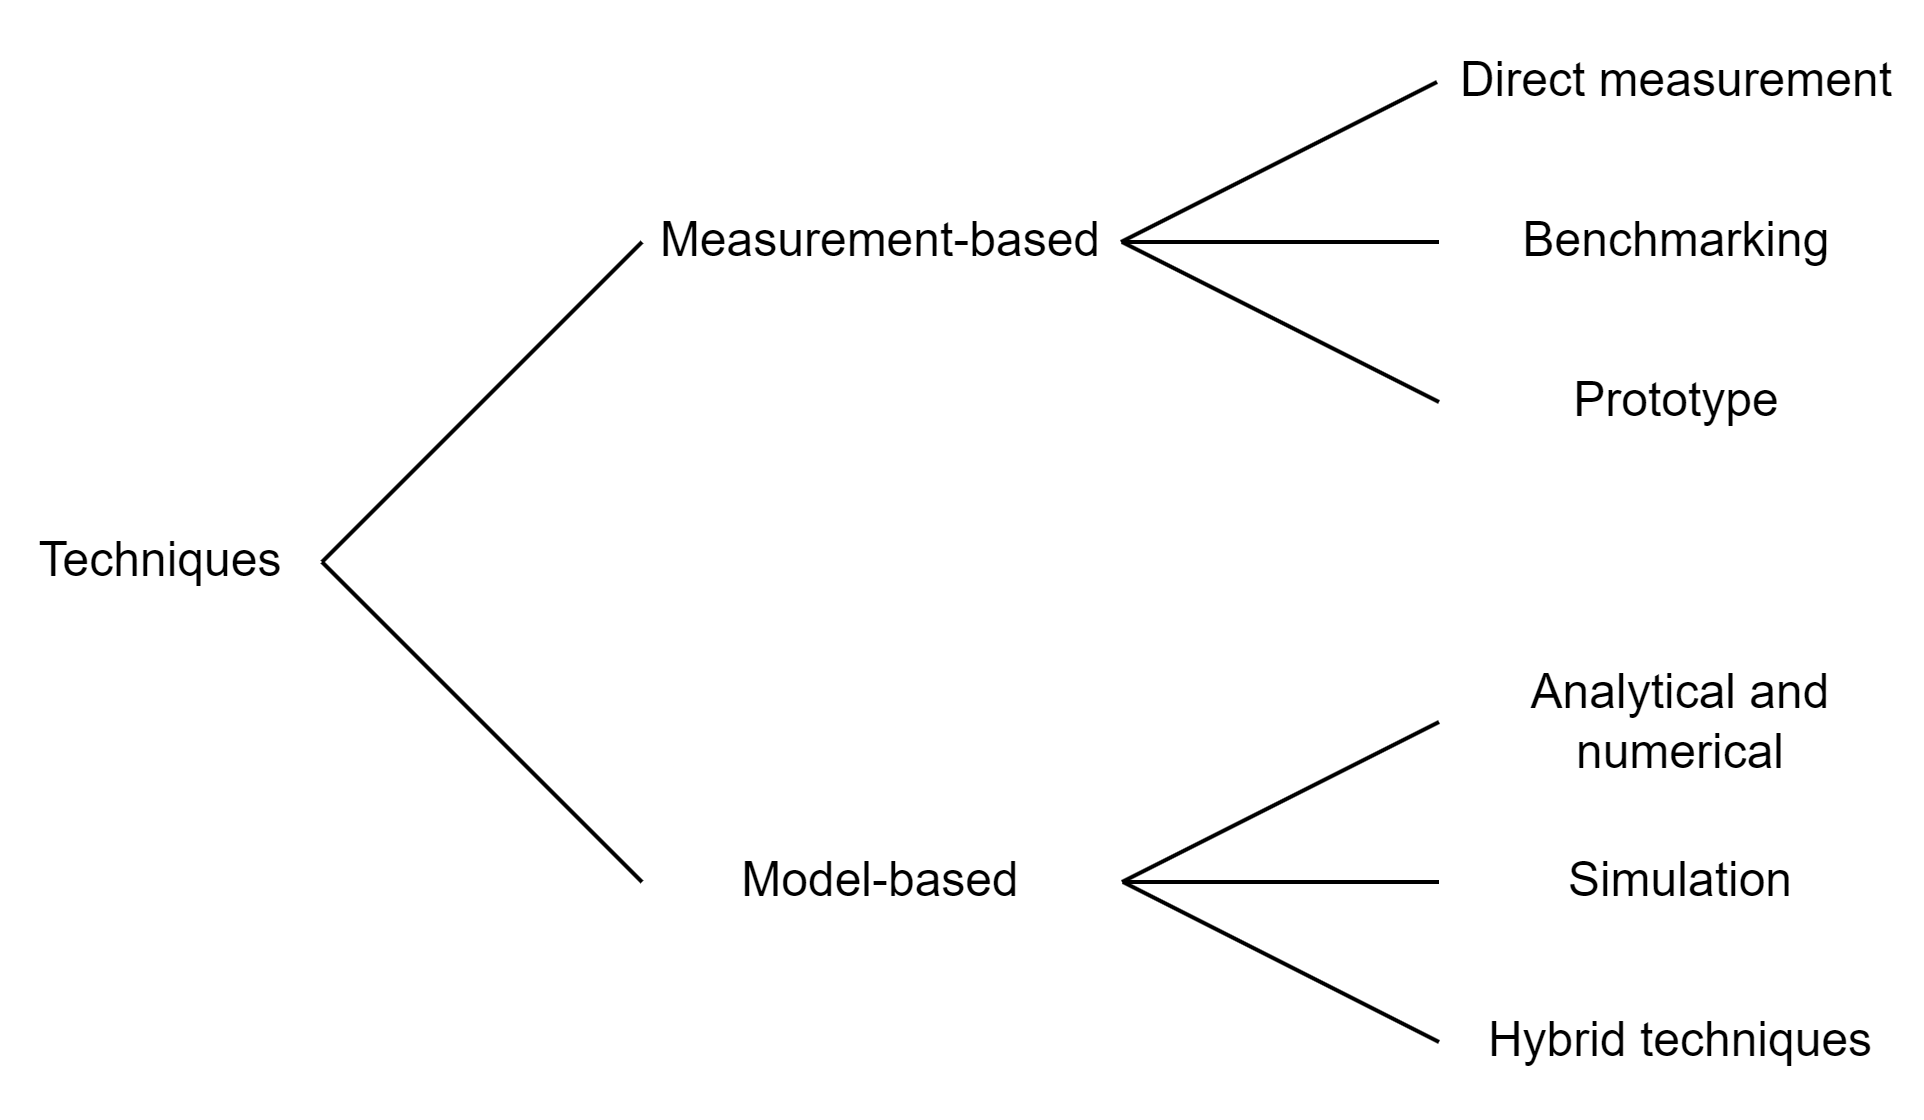
\includegraphics[width=0.5\linewidth]{images/eva.png}
    \caption{Quality evaluation techniques}
\end{figure}

\subsection{Model-based approach}
Given the complexity of systems, abstraction is necessary, achieved through the use of models. 
Frequently, models become the primary tool for handling these complexities, especially during phases like design. 
They guide design decisions by extracting essential aspects of system behavior from the intricate details.

\begin{definition}[\textit{Model}]
    A model serves as a simplified representation of a system, capturing its essential features while being less complex than the actual system.
\end{definition}
It enables making predictions and evaluations about the system's behavior.
\begin{figure}[H]
    \centering
    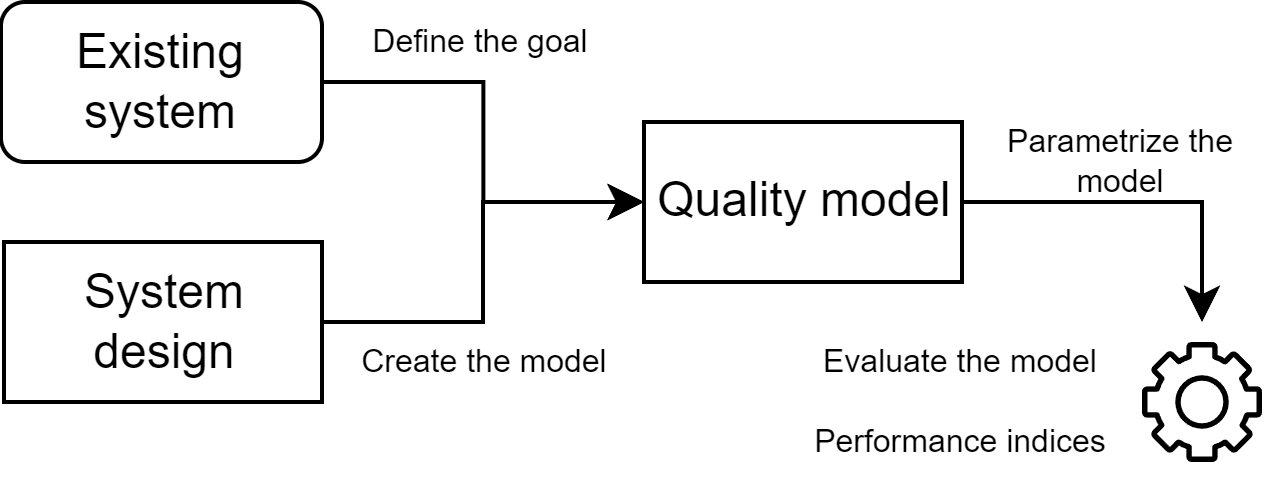
\includegraphics[width=0.5\linewidth]{images/model.png}
    \caption{Model definition}
\end{figure}

The main model-based approaches include:
\begin{itemize}
    \item \textit{Analytical and numerical techniques}: these methods rely on mathematical techniques, often utilizing results from probability theory and stochastic processes. 
        While they are highly efficient and precise, they are only available for very specific cases due to their limitations.
    \item \textit{Simulation techniques}: these methods involve replicating the behavior of the model. 
        They are versatile but may lack accuracy, particularly in scenarios involving rare events.
        Additionally, achieving high accuracy can result in lengthy solution times.
    \item \textit{Hybrid techniques}: these approaches combine analytical or numerical methods with simulation, leveraging the strengths of both to address various aspects of the system.
\end{itemize}